\frame{\frametitle{Un poco de turbulencia HD}
\begin{equation*}\label{eq2:N-S}
  \frac{\partial \vec{v}}{\partial t} + \vec{v}\cdot\nabla\vec{v} =
  -\frac{1}{\rho}\nabla p + \nu\nabla^2 \vec{v},
\end{equation*}

\begin{itemize}
\item Viscosidad presente $\Rightarrow$ decaimiento energético distintivo
\item Taylor, von Karman, Howarth, Kolmogorov.
\end{itemize}

  \begin{columns}
    \column{0.5\textwidth}
    \begin{minipage}[t]{1\textwidth}
      \begin{center} 
        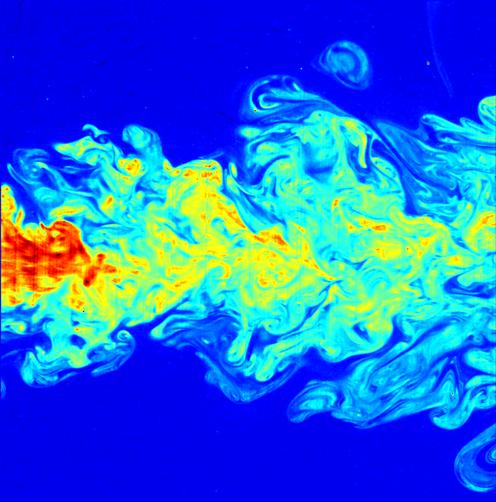
\includegraphics[width=0.6\columnwidth]{extra/turbulence1.jpg}
      \end{center}
    \end{minipage}
    \column{0.5\textwidth}
    \begin{minipage}[t]{1\textwidth}
      \begin{center}
        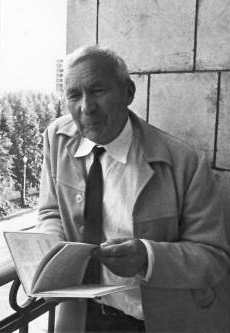
\includegraphics[width=0.5\columnwidth]{extra/turbulence2.jpg}
      \end{center}
    \end{minipage}
  \end{columns}
}
\note[itemize]{
\item Turbulencia MHD $\neq$ HD.
\item $B$ de gran escala juega rol significativo.
\item Influencia pequeñas escalas.
\item Entonces más escalas temporales influenciando.
\item Entonces, cascada más compleja
\item
\item Sin embargo, HD vale la pena como intro.
\item
}




\frame{\frametitle{Un poco de turbulencia HD}
El proceso de transferencia de energía:
\begin{center}
  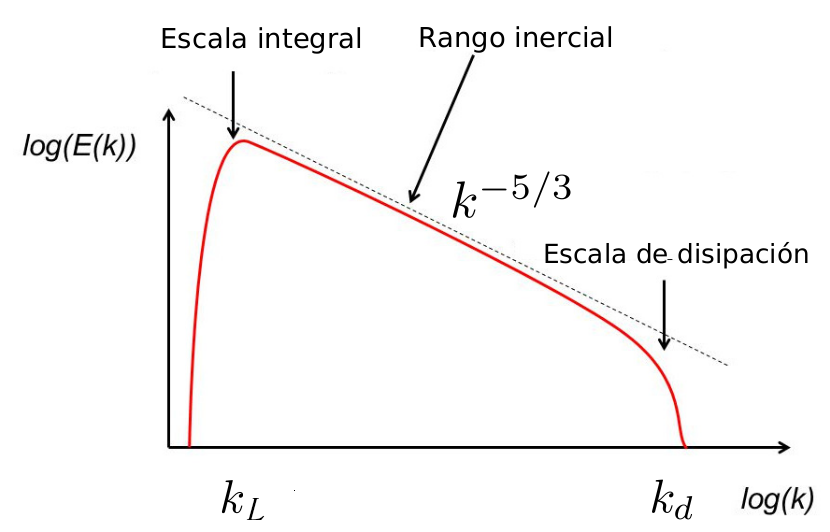
\includegraphics[width=0.4\columnwidth]{Fundamentos/EspectroKolmogorov.png}
\end{center}

Para poder inferir el espectro en el rango inercial, es necesario
estimar la magnitud de las correlaciones de la función de
transferencia (triple correlación), y en consecuencia la escala
temporal del decaimiento de las correlaciones de las funciones de
transferencia, $\tau_T(k)$.\vfill

Por argumentos dimensionales, $\epsilon = \overline{C} \tau_T(k) k^4 E^2(k)$. \vfill

El espectro de Kolmogorov, $E(k) = C_K \epsilon^{2/3} k^{-5/3}$, se
recupera proponiendo $\tau_T(k) = \tau_{nl}(k)$, donde este último
tiempo es el tiempo característico de los \emph{eddies}, $\tau_{nl}(k)
= \ell/v_k$.
}
\note[itemize]{
\item Fuerza aplicada a escala $L$ (ingresa energía)
\item Movimiento inestable y pierde energía a escalas vecinas más pequeñas, sin disiparse directamente en forma de calor
(transferencia local de energía).
\item Proceso repetido hasta escala de disipación $l_d$ (la escala de Kolmogorov), donde la
energía transferida se dispersa en forma de calor por acción
viscosa.
\item
\item EFECTOS. STRAINING Y SWEEPING.
}


\frame{\frametitle{Un poco de turbulencia HD: \emph{straining} y \emph{sweeping}}
\begin{itemize}
\item El espectro de Kolmogorov clásico se basa en la representación de la cascada
energética, causada por la interacción de \emph{eddies} de casi el mismo tamaño.
\item Las interacciones consisten en movimientos de \underline{\emph{straining}}.
\item También está presente la interacción entre escalas grandes y pequeñas, mediante
un movimiento de barrido (\underline{\emph{sweeping}}), pero no involucra transferencia energética
significativa en el espacio de Fourier.
\item En las correlaciones temporales, el \emph{sweeping} cobra gran importancia.
\item También cobra importancia para los momentos de orden más alto.
\end{itemize}
}
\note[itemize]{
\item 1) Cascada energética, similar a saltos de agua.
\item 2) Un vórtice se estira, produciendo grad de velocidades que distorsiona otros vórtices.
\item 3) Los remolinos grandes arrastran a los pequeños, pero no los deforman.
\item 4) \emph{Frozen turbulence}
\item 5) Funciones de estructura, espectro de energía cinética, etc.
\item 5) Entonces, no influye el espectro, pero es importante.
\item
\item AGREGARSE EFECTOS EXTRA
}


\frame{\frametitle{Un poco de turbulencia HD}
Ahora bien, ?`cómo pueden agregarse los efectos de otras escalas
temporales en una teoría simple de espectros turbulentos? Una
posibilidad es reescribir la tasa de transferencia espectral:
$\epsilon = \Pi(k) = \frac{u_k^2}{\tau_{sp}}$\vfill

Aquí, el tiempo de transferencia espectral de energía puede escribirse
como $\tau_{sp} = \tau_{nl}^2/\tau_T(k)$. Desarrollando diferentes
aproximaciones para $\tau_T$ de la triple correlación, es posible
obtener una variedad de modelos para los espectros de turbulencia.\vfill

%% Es más, este enfoque fenomenológico concuerda con las conclusiones de
%% las diversas teorías de clausura de la turbulencia: la ley espectral
%% de potencias viene determinada por la elección de una escala temporal
%% relacionada con las transferencias no lineales de energía.

Resulta razonable buscar un tratamiento fenomenológico del espectro
MHD para entender la variedad de conclusiones que pueden ser
aplicables al espacio y a plasmas astrofísicos.
}
\note[itemize]{
\item 2) Esto se condice con conclusiones de las teorías de clausura.
\item
\item TURBULENCIA MHD
}




\frame{\frametitle{Turbulencia MHD}
\begin{center}
$\frac{\partial \vec{v}}{\partial t} + \vec{v} \cdot \nabla\vec{v} = -\frac{1}{\rho} \nabla p + \frac{1}{4\pi\rho} \left(\nabla\times\vec{B}\right)\times\vec{B} + \nu \nabla^2 v$ \\
$\frac{\partial \vec{B}}{\partial t} = \nabla \times \left(\vec{v}\times\vec{B}\right) + \mu \nabla^2 \vec{B}$
\end{center}\vfill

El modelo MHD es frecuentemente aplicado al espacio y a plasmas
astrofísicos. \vfill

Cuando se tienen observaciones experimentales
disponibles (viento solar), se puede ver que el rango inercial es
amplio, por lo que el rango de inyección de energía se encuentra bien
separado en escala del rango disipativo, y resulta posible inferir un
Reynolds efectivo.
}
\note[itemize]{
\item Ecs. de momentos y de inducción magnética
}



\frame{\frametitle{Turbulencia MHD}
\begin{itemize}
\item El campo magnético puede ser escrito como $\vec{B} = \vec{B}_0 + \vec{b}$.
\item El campo magnético de gran escala permite y respalda la propagación de ondas
hidromagnéticas (ondas de Alfv\'en).
\item Estas ondas son fluctuaciones transversales a $\vec{B}_0$, propagándose
en su misma dirección a la velocidad de Alfv\'en $V_A =
B_0/\sqrt{4\pi\rho}$, y siguiendo la relación de dispersión $\omega
= \pm V_A k_\parallel$.
\item Las fluctuaciones de pequeña escala sufren un efecto
similar al \textit{sweeping} debido a la propagación de ondas de
Alfv\'en (\textit{sweeping} magnético).
\item Además, el \emph{sweeping} juega un papel importante, pues
$\vec{B}_0$ no puede ser removido por transformaciones de Galileo $\Rightarrow$ anisotropía.
\item Esto introduce una nueva escala temporal, complejizando la turbulencia.
\end{itemize}
}
\note[itemize]{
\item 1) Parte uniforme $\vec{B}_0$ (DC) o que varía muy suavemente
(campo magnético medio local), más fluctuaciones de pequeña escala $\vec{b}$
\item
\item TEORÍAS FENOMENOLÓGICAS
}





\frame{\frametitle{Turbulencia MHD}
Hay varias teorías fenomenológicas, dependiendo de la escala temporal dominante:
\begin{itemize}
\item Iroshnikov (1964) y Kraichnan (1965): $\tau_T = \tau_A \Rightarrow E(k) \sim k^{-3/2}$
\item Fyfe y Montgomery (1976): $\tau_T = \tau_{nl} \Rightarrow E(k) \sim k^{-5/3}$
\item Matthaeus y Zhou (1989): $\frac{1}{\tau_T(\vec{k})} = \frac{1}{\tau_{nl}(\vec{k})} + \frac{1}{\tau_A(\vec{k})}$
\end{itemize}
}
\note[itemize]{
\item $\tau_T(k)$: escala temporal del decaimiento de las correlaciones
de las funciones de transferencia.
\item I-K: Para $B_0$ fuerte.
\item F-M: Vale Kolmogorov
\item M-Z: Respeta los casos límites
}



\frame{\frametitle{Turbulencia MHD}
Más allá de los detalles (presentes en la tesis), la conclusión es que
con MHD el análisis se complejiza aún más.\vfill

En cualquier caso, las distintas escalas temporales tienen un rol
influyente en la transferencia de energía, las cascadas, la no
localidad y la anisotropía.\vfill

Los movimientos de \textit{straining} son dominantemente locales en
escala, dado que las distorsiones no lineales son más efectivas para
interacciones entre \textit{eddies} de aproximadamente el mismo
tamaño.\vfill

Por su parte, el barrido debido a propagación de ondas Alfv\'enicas
introduce un nuevo nivel de no-localidad en MHD y una fuerte tendencia
a que la transferencia espectral ocurra anisotrópicamente respecto de
la dirección del campo magnético.
}
\note[itemize]{
\item
\item ESPECTROS DE FRECUENCIAS
}



\frame{\frametitle{Espectros de frecuencias}
\begin{itemize}
\item En los '70, la investigación de la turbulencia hidrodinámica
se dirigió al estudio del tiempo de descorrelación del campo de
velocidades.
\item Además de las correlaciones espaciales, también cobró interés el estudio del
espectro en frecuencias más allá de la hipótesis de Taylor.
\item La conclusión principal fue que el \textit{sweeping} aleatorio domina
la descorrelación temporal en el rango inercial para el caso hidrodinámico.
\end{itemize}
}
\note[itemize]{
\item 2) correlaciones de dos tiempos y un punto espacial
}


\frame{\frametitle{Espectros de frecuencias}
\begin{itemize}
\item Nuevamente, el caso MHD resulta mucho más complejo, quedando aún
muchas preguntas acerca de cuál es la escala temporal dominante de la
descorrelación temporal.
\item Servidio \emph{et al} (2011) realizaron un estudio para
analizar a descorrelación temporal para el caso de turbulencia MHD
isotrópica.
\item El resultado principal: la descorrelación temporal en MHD es gobernada por
interacciones no locales, pero no pudieron
distinguir entre los efectos del \emph{sweeping} y de la distorsión
Alfv\'enica.
\end{itemize}
\begin{center}
  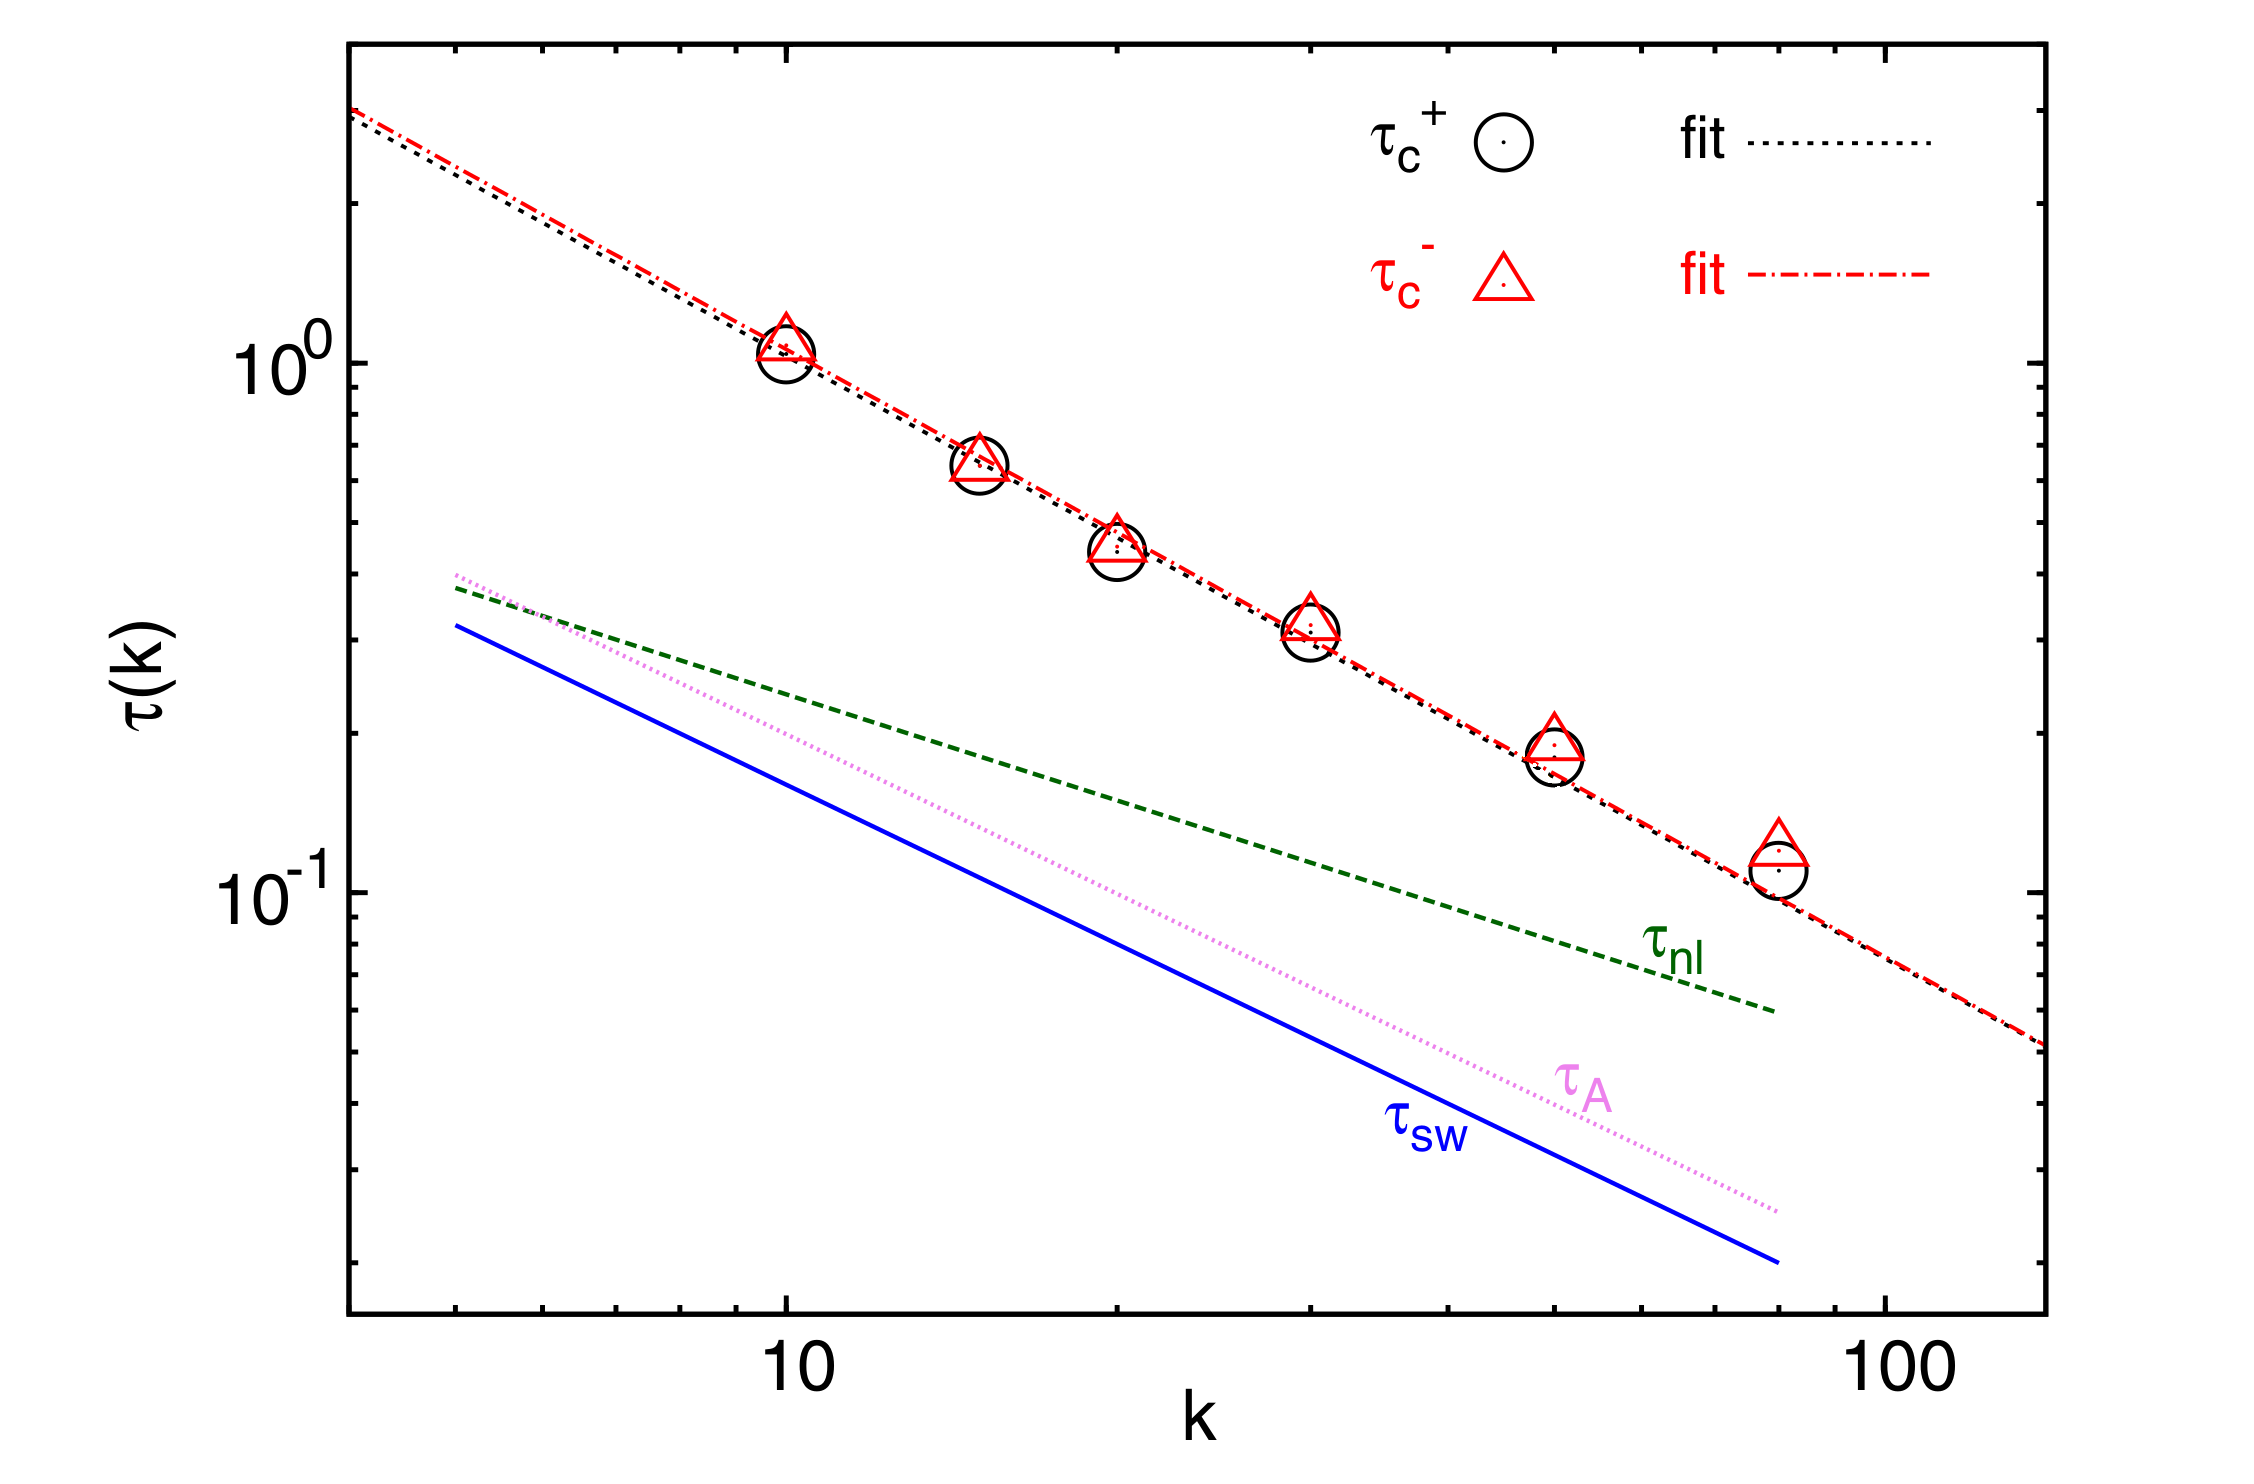
\includegraphics[width=0.4\columnwidth]{Fundamentos/ServidioDescorrelacion.png}
\end{center}
}
\note[itemize]{
\item 2) en este caso, \emph{sweeping} aleatorio y propagación de Alfv\'en
\item figura: tiempos de decorrelación
\item
\item CASO DE ESTUDIO
}
